\section{Cassandra Speculative Decoding Algorithm}
\label{section_4}

\subsection{Overview of Cassandra Algorithm}
\label{section_4_1}
To address the limitations of conventional speculative decoding in edge environments, Cassandra is designed around two key objectives: resource efficiency and low-batch performance.

First, Cassandra targets reliable operation under constrained compute and memory budgets. Approaches that require additional training are impractical for widespread deployment on edge devices, and maintaining a separate draft model introduces non-negligible memory capacity overhead. To overcome these issues, Cassandra adopts a training-free self-speculative decoding framework, eliminating the need for additional training while avoiding duplication of model parameters.

Second, Cassandra is optimized for performance in low-batch inference scenarios. Prior self-speculative decoding methods primarily focus on optimizing the attention layer and KV cache. Also, for computational efficiency on GPU, they usually adopt coarse-grained methods such as structured pruning or layer skipping to generate the draft model. However, such approaches are not sufficient in low-batch regimes. When the batch size is small and sequence lengths are moderate, the dominant bottleneck in the decode stage shifts from attention to the weight loading of the feed-forward network (FFN) layers. Therefore, improving performance in this setting requires not only optimizing attention-related operations but also effectively reducing the memory footprint of FFN weights. Furthermore, since the decode stage is typically memory-bound, minimizing data movement is more critical than improving raw computational efficiency.

Figure~\ref{fig_4_1} illustrates the core design of Cassandra. The weights and KV cache of the original model are first transformed into a specialized format and partitioned into two components: \textbf{speculation data} and \textbf{verification data}.

During draft inference, only the speculation data is loaded and reconstructed into the original format using zero-padding. Although the resulting draft model is executed using standard floating-point units and does not reduce arithmetic complexity, it significantly lowers memory bandwidth requirements, enabling faster execution.

During target model inference, both the speculation and verification data are loaded and fully reconstructed to recover the original model representation. Unlike conventional speculative decoding methods~\cite{speculativesampling, eagle3}, Cassandra does not require an independent draft model. Instead, the draft model operates on a strict subset of the original model parameters, allowing speculative decoding to be performed without additional memory capacity overhead.

% To mitigate the drawbacks of conventional speculative decoding on edge devices, Cassandra is designed with a primary focus on two key areas.

% One focus of our design is to ensure reliable operation even in environments with constrained computing and memory resources. We assessed that the methods necessitating additional training are unsuitable for widespread adoption on edge devices. Furthermore, the memory capacity overhead incurred by separately storing a draft model presents a non-negligible problem for resource-constrained devices. Consequently, we designed Cassandra with a training-free self-speculative decoding architecture.

% The second focus is on performance enhancement in low-batch environments. Many previously self-speculative decoding methods primarily focus on attention layer and KV cache optimization. Also, for computational efficiency on GPU, they usually adopt coarse-grained methods such as structured pruning or layer skipping to generate the draft model. However, improving performance in low-batch scenarios requires considering additional factors. First, when the batch size is small and the sequence length is not very long, the core bottleneck in the decode stage arises from the weight loading process in the Feed-Forward Network (FFN) layer, rather than the attention layer and the KV cache. Considering this, for low-batch self-speculative decoding, it becomes crucial to effectively reduce the weight of the FFN layer in addition to optimizing the attention layer. Furthermore, given that the decode stage is typically memory-bound, it is more effective to design algorithms that prioritize minimizing the size of the data being loaded rather than focusing solely on compute efficiency.

% Figure~\ref{fig_4_1} illustrates the basic concept of Cassandra. First, the original model's weight and KV cache undergo a series of format transformation processes and are divided into two groups: ~\textbf{speculation data} and ~\textbf{verification data}.

% Afterward, when we perform draft model inference, we only load the speculation data and decode it to the original data format with zero-padding. In this case, the decoded draft model is also computed by using a floating-point arithmetic unit and cannot make computation more efficient. However, this model requires significantly less memory bandwidth, allowing it to be executed much faster than the original model.

% After the draft model generates a few tokens, when we perform target model inference, we load both the speculation data and the verification data, decode, and restore them to the original floating-point format. Unlike traditional speculative decoding methods~\cite{speculativesampling, eagle3}, since the data used for draft model inference is physically a subset of the data used for the target model, we can perform speculative decoding without incurring any memory capacity overhead.

%%%%%%%%%%%%%%%%%%%%%%%%%%%%%%%%%%%%%%%%%%%%%%%%%%%%%%%%%%%%%%%%%%%%%
\begin{figure}[t!]
\centering
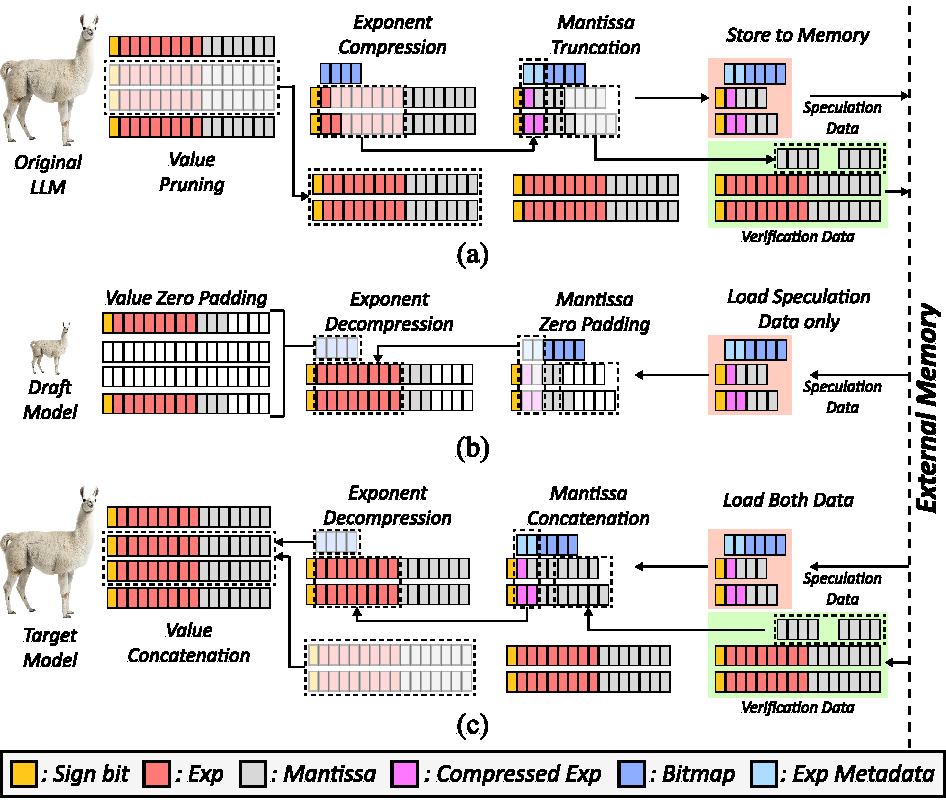
\includegraphics[width=\colimgwidth]{Figures/4_1_Cassandra_Concept.pdf}
\caption{Visualization of Cassandra Algorithm. (a) Cassandra's initial format transformation flow (b) Draft model inference (c) Target model inference}
\label{fig_4_1}
\end{figure}
%%%%%%%%%%%%%%%%%%%%%%%%%%%%%%%%%%%%%%%%%%%%%%%%%%%%%%%%%%%%%%%%%%%%%%


\subsection{Step-by-Step Format Transformation Flow in Cassandra}
\label{section_4_2}
In this section, we elaborate on how the original model undergoes a format transformation process to be partitioned into speculation data and verification data. In the subsequent paragraphs, the data selected through the pruning or truncation process constitute the speculation data. Unlike lossy compression, the data that are not selected during this process are not discarded; instead, they become the verification data and are utilized for target model inference.

~\textbf{Unstructured Value Pruning.} First, Cassandra performs unstructured pruning on the weights and KV caches of the original model. Regarding weights, we employ the activation-aware weight pruning technique proposed in Wanda~\cite{Wanda}. Leveraging the observation that activations exhibit large magnitudes in specific channels regardless of the input, Wanda computes the L2 norm of activations using calibration data and multiplies the resulting values element-wise by the weights to determine importance scores for pruning.

In contrast to weights, Cassandra applies per-token magnitude-based pruning for the KV cache. According to Mustafar~\cite{Mustafar}, this approach is highly effective for Key caches due to the presence of prominent channel-wise outliers. Although Value caches do not exhibit a similarly distinct outlier distribution, per-token pruning remains effective, as it is functionally equivalent to output-aware pruning within the attention mechanism.

Since these methods are designed primarily to preserve the output of each layer, they are more advantageous in terms of acceptance rate relative to compression ratio compared to structured pruning, which utilizes pre-determined masks for computational efficiency. Also, both methods involve minimal to negligible calibration costs, aligning well with Cassandra's design philosophy of being training-free.

~\textbf{Mantissa Truncation.} In addition to pruning, we further reduce the representation cost of each value by truncating mantissa bits. While quantization is the conventional approach for reducing bit-width, we instead adopt a naive mantissa truncation scheme. This choice significantly lowers the overhead of format reconstruction compared to quantization. Furthermore, unlike quantization, which alters the numerical representation, mantissa truncation preserves a subset of the original bits. As a result, the draft model can be interpreted as a strict subset of the target model, which is a key property that enables Cassandra to avoid additional memory capacity overhead.

% The combined use of value pruning and mantissa truncation is crucial for a higher compression ratio. Figure~\ref{fig_4_2}(a) shows the acceptance rate versus compression ratio when using value pruning alone, mantissa truncation alone, and when using both algorithms together. As the figure shows, the combined scheme achieves a significantly higher acceptance rate versus compression ratio than either single scheme. Figure~\ref{fig_4_2}(b) shows the ideal performance gain measured on the NPU simulator for each case. This demonstrates that higher compression ratios with maintained accuracy significantly boost overall system performance.

\textbf{Exponent Compression.} The application of the two aforementioned algorithms still results in limited compression ratios. This limitation stems from the uncompressed exponent, which accounts for 50\% of the bit-width in the standard BFloat16 datatype. Therefore, to achieve significant performance improvements, additional compression must be applied.

%%%%%%%%%%%%%%%%%%%%%%%%%%%%%%%%%%%%%%%%%%%%%%%%%%%%%%%%%%%%%%%%%%%%%%%%%%%%%%%
\begin{figure}[t]
\centering
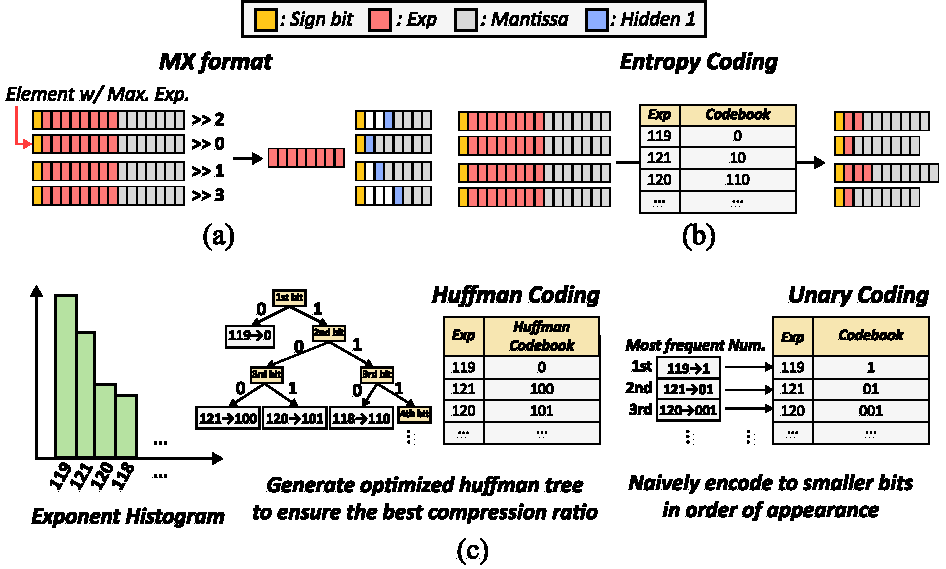
\includegraphics[width=\colimgwidth]{Figures/4_3_Exponent_Compression.pdf}
\caption{(a) MX format, (b) Entropy Coding, (c) Huffman and Unary Coding}
\label{fig_4_2}
\end{figure}
%%%%%%%%%%%%%%%%%%%%%%%%%%%%%%%%%%%%%%%%%%%%%%%%%%%%%%%%%%%%%%%%%%%%%%%%%%%%%%%

One possible approach is to adopt the MX format~\cite{microscaling}, in which multiple floating-point values share a common exponent. This format has been widely utilized in deep learning training and inference due to its efficiency. However, converting a model trained in a standard floating-point format into MX format inevitably introduces some degree of accuracy degradation. Although this degradation is often small, we argue that a complementary approach with no risk of accuracy loss is also desirable. From this perspective, we identify entropy coding as a suitable method for lossless exponent compression.


Entropy coding is a lossless compression technique that assigns variable-length codes based on the frequency distribution of values. Shannon entropy~\cite{ShannonEntropy} provides a theoretical lower bound on the average number of bits required to represent such data. Previous work~\cite{dfloat11} has shown that the exponent values of BFloat16-trained weights exhibit a Shannon entropy of approximately 2.6 bits. As illustrated in Figure~\ref{fig_4_3}(a), we further observe that the exponent distribution of the KV cache also has low entropy, averaging around 2.7 bits. These results suggest that, by applying appropriate entropy coding to both weights and KV cache, it is theoretically possible to achieve a lossless reduction of more than 5 bits.

% Entropy coding is a lossless data compression technique that performs variable-length coding based on the frequency of each unique value in a dataset. Shannon entropy~\cite{ShannonEntropy} quantifies the theoretical minimum number of bits by which data can be compressed using entropy coding. Previous research~\cite{dfloat11} has shown that exponent bits, when isolated from weights trained in BFloat16, exhibit a Shannon entropy of approximately 2.6 bits. 
% As shown in Figure~\ref{fig_4_3}(a), we also confirmed that the Shannon entropy obtained from the exponent of the KV cache is very low, averaging at only 2.7 bits. This implies that if we apply appropriate entropy coding to both the LLM's weight and the KV cache, we can theoretically achieve a lossless reduction of more than 5 bits.

Among entropy coding techniques, Huffman coding~\cite{HuffmanCoding} is one of the most widely used methods, and several prior studies~\cite{dfloat11, Huff-LLM} have explored its application to LLM compression. However, implementing Huffman decoding efficiently on xPUs presents significant challenges. A conventional LUT-based decoding approach~\cite{Huffman-GPU-LUT} requires a lookup table with $2^N$ entries, where $N$ denotes the number of unique symbols. In LLMs, where $N$ can be as large as 32, such an approach becomes impractical. While hierarchical codebooks~\cite{dfloat11} can mitigate this issue, they introduce additional decoding complexity and latency. As a result, the overhead of decoding may outweigh the benefits of compression, leading to worse overall system performance compared to the BFloat16 baseline.

% One of the most widely used entropy coding methods is Huffman coding~\cite{HuffmanCoding}, and several prior studies~\cite{dfloat11, Huff-LLM} have attempted to leverage this method for LLM compression. However, if we use a traditional LUT-based approach~\cite{Huffman-GPU-LUT} for performing Huffman decoding on xPUs, we need to use a LUT with $2^N$ indices, where $N$ is the number of unique exponents. This is practically infeasible for LLMs where $N$ can be as large as 32. While some research~\cite{dfloat11} has attempted to overcome this with a hierarchical Huffman codebook, this further increases the decoding overhead. In such cases, despite the compression, the prolonged decoding latency results in worse system performance compared to the BFloat16 baseline.

%%%%%%%%%%%%%%%%%%%%%%%%%%%%%%%%%%%%%%%%%%%%%%%%%%%%%%%%%%%%%%%%%%%%%%%%%%%%%%%
\begin{figure}[t]
\centering
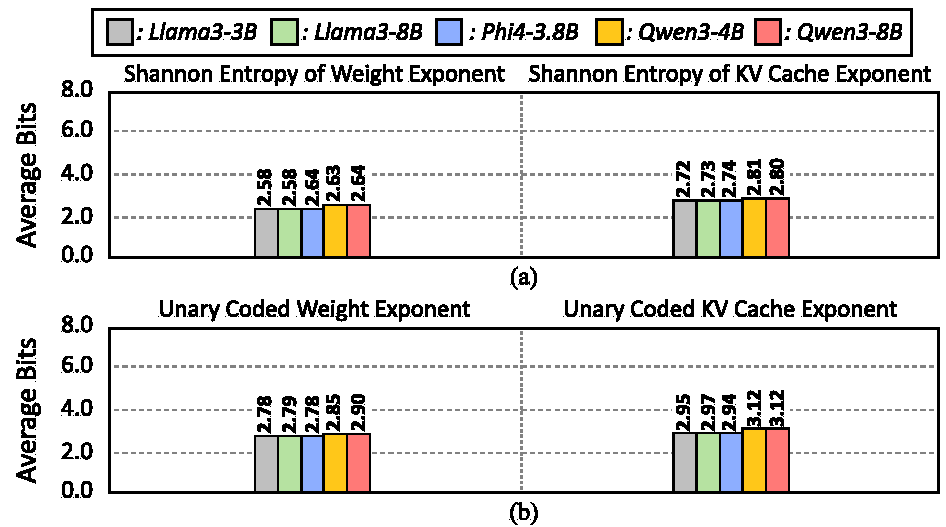
\includegraphics[width=\colimgwidth]{Figures/4_3_Shannon_Entropy.pdf}
\caption{(a) Average Shannon entropy of exponent in weight and KV cache. (b) Average exponent bits of unary-coded weights and KV cache}
\label{fig_4_3}
\end{figure}
%%%%%%%%%%%%%%%%%%%%%%%%%%%%%%%%%%%%%%%%%%%%%%%%%%%%%%%%%%%%%%%%%%%%%%%%%%%%%

To overcome this issue, we propose a much simpler method: Unary coding can be a solution for low-overhead lossless exponent compression. Unary coding is a method of assigning codes simply by increasing the length by one, corresponding to the frequency of a particular element. In Cassandra, unary coding is implemented by encoding numbers in a format where $N$ consecutive zeros are followed by a final one, such as $1, 01, 001,$ and so on. Exponents that appear more frequently are assigned fewer bits. The key advantage of this method lies in its explicit boundary representation: every codeword is terminated by a \textbf{1}, allowing unambiguous identification of code boundaries directly from the compressed bitstream. As a result, unlike conventional entropy coding schemes, which often require sequential parsing or LUT-based decoding, unary coding can be implemented using simple, fully parallel digital logic.

% This method is extremely simple and offers the advantage that the decoding process can be fully accelerated using a digital logic circuit without sequential LUT lookups. Because unary coding does not offer mathematically optimal compression, it has not been frequently utilized in conventional compression research.

As shown in Figure~\ref{fig_4_3}(b), we confirmed that unary coding can achieve an average exponent compression of 2.85 bits. Although its compression efficiency is slightly lower than that of Huffman coding, it still provides a substantial improvement over the original floating-point representation. Also, from the perspective of overall system performance, the reduction in decoding overhead achieved by using unary coding provides a more positive impact than the slight loss in compression ratio.

Unary coding preserves full numerical accuracy, whereas the MX format offers higher compression efficiency at the cost of slight accuracy degradation. Consequently, neither approach can be considered universally superior. To accommodate this trade-off, Cassandra supports both methods. We refer to the unary coding-based, lossless configuration as Cassandra-1, and the MX-based, higher-performance configuration with minor accuracy loss as Cassandra-2. This design enables users to select the most appropriate configuration based on their accuracy and performance requirements. Although mantissa truncation was introduced earlier for clarity, exponent compression is applied prior to mantissa truncation in the actual algorithm, as illustrated in Figure~\ref{fig_4_1}.
%%

 
% \vspace{-0.05in}
% \begin{equation}
%  M = \max(|\text{Min}|, |\text{Max}|), \; \ \sigma = \frac{M}{2^{m-1} - 1}, \; \  Q(x) = \text{round} \left( \frac{x}{\sigma} \right)
% \label{eq_4_1}
% \end{equation}
% \vspace{-0.05in}

% \begin{figure}[t!]
% \centering
% \includegraphics[width=\colimgwidth]{Figures/4_2_Bit_Level_Algorithm_2.pdf}
% \caption{Bit Level Algorithm Flow}
% \label{fig_1_1}
% \end{figure}


% \subsection{Shared Memory Space for Draft Model}
% \label{section_4_2}

% In the context of **self-speculative decoding**, the data for our generated **draft model** originates from the **target model**. While methods like **quantization** fundamentally alter the target model's bits, a draft model created using **pruning** or **bit truncation** still retains some of the target model's original bits.

% Cassandra leverages this fact to develop a novel storage scheme that allows the draft model to be stored **without a separate memory space** for its weights and KV cache. Unlike general **lossy compression algorithms** that completely discard low-importance data, Cassandra uses the previously introduced compression algorithm as a metric to divide the model's weights and KV cache into two groups: the **speculation group** and the **verification group**.

% The **speculation group** consists of the relatively **important values** selected from the weights and KV cache via the algorithm introduced in Section 4.2. The **verification group** contains values that are relatively **less important** but are necessary for accurate inference. When attempting to generate tokens quickly using the draft model, we only fetch the **speculation group**, apply **zero padding** to the rest, and perform the computation. Conversely, if we want to verify the $N$ tokens generated this way using the target model, we read all data from both the speculation and verification groups and perform **decompression at once**. In both cases, the computation is performed using the **same floating-point arithmetic units**. However, since the **Attention** and **FFN (Feed-Forward Network)** of the **low-batch decode stage** we target are **memory-bound** on the xPU, and the amount of data included in the speculation group is significantly smaller than the total data size, this method achieves a sufficient performance improvement.

% This **group division** method, combined with **memory space sharing** between the target and draft models, allows us to perform speculative decoding **without any additional memory space** for the draft model. This greatly aids in generating long tokens. For example, comparing Cassandra with speculative decoding using Llama3-8B and Llama3-1B, Cassandra can generate N\% more tokens compared to Llama3-1B.





\subsection{Design Space Exploration of Cassandra Algorithm: Trade off between Acceptance Rate and Compression Ratio}
\label{section_4_3}
In LLM inference with lossy compression, a higher compression ratio typically results in a larger accuracy drop. Thus, the acceptable accuracy drop determines the final compression ratio. For this reason, combining multiple lossy compression algorithms is often avoided in standard LLM inference scenarios.

However, speculative decoding uses the target model for verification, essentially eliminating the accuracy drop, regardless of the draft model's compression ratio. Instead, in this case, the compression ratio and the acceptance rate are in a trade-off relationship. At this point, the draft model does not need to generate the correct complete sentence by itself; it only needs to retain the ability to predict a few tokens correctly. In this case, the conditions for generating the optimal draft model differ from the methods used in lossy compression.

Figure~\ref{fig_4_4} shows the acceptance rate versus compression ratio when using the Deepseek-R1-Distillated-Llama-8B model, with the draft model created using value pruning and mantissa truncation separately, and when using both schemes together. At this point, using value pruning and mantissa truncation together demonstrates a robust acceptance rate compared to using either method alone. This result demonstrates that Cassandra's format transformation method, which integrates multiple schemes, is suitable for self-speculative decoding.

%%%%%%%%%%%%%%%%%%%%%%%%%%%%%%%%%%%%%%%%%%%%%%%%%%%%%%%%%%%%%%%%%%%%
\begin{figure}[t]
\centering
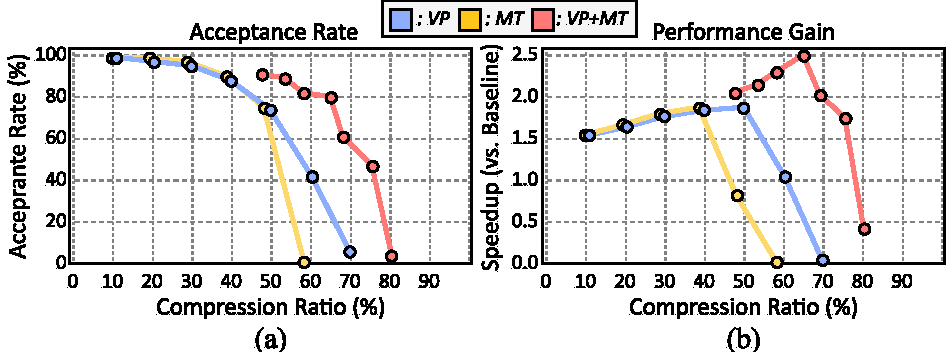
\includegraphics[width=\colimgwidth]{Figures/4_2_mantissa_truncation_graph.pdf}
\caption{(a) Acceptance rate according to compression ratio($\gamma$=5). (b) Ideal performance improvement compared to baseline. VP means value pruning, MT means mantissa truncation, VP+MT means applying both schemes.}
\label{fig_4_4}
\vspace{-1.0em}
\end{figure}
%%%%%%%%%%%%%%%%%%%%%%%%%%%%%%%%%%%%%%%%%%%%%%%%%%%%%%%%%%%%%%%%%%%%%


% The draft model generation process in **Cassandra** might seem like an extension of other lossy compression methods. However, Cassandra utilizes a **different criterion** than conventional lossy compression when deciding the **sparsity ratio** or **truncation bits**. In existing lossy compression techniques like quantization and pruning, the primary criterion for setting the compression ratio is **accuracy**, such as **perplexity** or **zero-shot accuracy benchmarks**. This is because if a model is compressed too aggressively, its accuracy drops to an unusable level, completely losing its language understanding capability.

% However, the situation is slightly different in **speculative decoding**. A draft model in speculative decoding only needs to maintain the ability to **probabilistically generate words similar to the original model** and does not require high-level language understanding. Therefore, the criterion for determining the compression ratio in this context should be the draft model's **acceptance rate**, not its accuracy.

% **Graph N** illustrates the expected performance based on the trade-off between the **compression ratio** and the **acceptance rate** for using sparsity, bit truncation, and a combination of both. Here, we assume that the LLM decode stage is perfectly **memory-bound**, and performance is proportional to memory load.

% We can derive two key insights from this graph. First, both sparsity and bit truncation have a sort of **inflection point** where the decrease in acceptance rate begins to accelerate. Consequently, achieving a sufficient compression ratio is **not possible** using only one method (sparsity or bit truncation).

% Second, while combining quantization and pruning is **not common** in general model lossy compression, using **multiple compression schemes together** can be beneficial for speculative decoding. In standard lossy compression, overly aggressive model compression is often avoided because the model becomes unusable if its language understanding falls below a certain level, even if the compression ratio increases. However, in speculative decoding, a **new sweet spot emerges** because even if the acceptance rate decreases, accuracy is maintained, and the draft model's latency also decreases. From this graph, we can see that when combining the two schemes, we can achieve an acceptance rate that is **N\% higher** for a given compression ratio compared to using either sparsity or bit truncation alone. This suggests that Cassandra's complex compression/decompression algorithm is an **effective method** for improving speculative decoding performance.